% Capítulo 1: arquitetura de Von Neumann.
\documentclass[border=4pt]{standalone}
\usepackage[utf8]{inputenc}
\usepackage[T1]{fontenc}
% Estilo comum dos fluxogramas e diagramas de blocos.
\usepackage{tikz}
\usetikzlibrary{arrows.meta, positioning, calc, shapes.geometric, shapes.misc}
\definecolor{navy}{RGB}{23,45,80}
\definecolor{laranja}{RGB}{250,110,29}
\definecolor{cinzalogo}{RGB}{107,114,126}
\definecolor{azul}{RGB}{205,222,247}
\tikzset{
  base/.style={draw=navy, line width=0.9pt, font=\sffamily\small, align=center, inner sep=4pt},
  terminal/.style={base, rounded rectangle, fill=laranja!45, draw=laranja, minimum width=20mm, minimum height=7mm},
  processo/.style={base, rectangle, fill=laranja!12, minimum width=28mm, minimum height=8mm},
  decisao/.style={base, diamond, aspect=2.2, fill=azul, inner sep=1pt, minimum width=30mm},
  es/.style={base, trapezium, trapezium left angle=72, trapezium right angle=108,
             fill=white, minimum width=26mm, minimum height=8mm, trapezium stretches body},
  fluxo/.style={-{Stealth[length=2.2mm]}, navy, line width=0.9pt},
  rotulo/.style={font=\sffamily\small\bfseries, text=navy},
  legenda/.style={font=\sffamily\scriptsize, text=cinzalogo},
  resposta/.style={font=\sffamily\scriptsize\bfseries, text=navy},
}

\usetikzlibrary{backgrounds}
\tikzset{
  bloco/.style={base, rectangle, rounded corners=2pt, fill=laranja!12, minimum height=9mm},
  cpu/.style={draw=navy, line width=1.2pt, rounded corners=4pt, fill=azul!40},
  barramento/.style={draw=navy, line width=3pt, cinzalogo},
  liga/.style={{Stealth[length=2mm]}-{Stealth[length=2mm]}, navy, line width=0.9pt},
}
\begin{document}
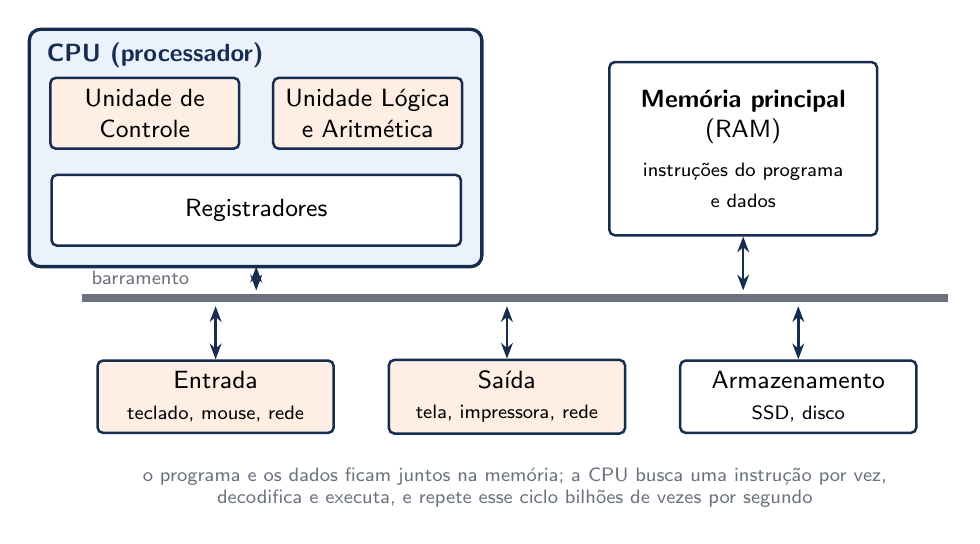
\begin{tikzpicture}
  % CPU com suas partes
  \node[bloco, minimum width=24mm] (uc) at (0, 0) {Unidade de\\Controle};
  \node[bloco, minimum width=24mm, right=4mm of uc] (ula) {Unidade Lógica\\e Aritmética};
  \node[bloco, minimum width=52mm, fill=white, below=3mm of $(uc.south)!0.5!(ula.south)$] (reg) {Registradores};
  \begin{scope}[on background layer]
    \draw[cpu] ($(uc.north west)+(-0.25, 0.6)$) rectangle ($(reg.south east)+(0.25, -0.25)$);
  \end{scope}
  \node[rotulo, anchor=north west] at ($(uc.north west)+(-0.15, 0.55)$) {CPU (processador)};

  % memória
  \node[bloco, minimum width=34mm, minimum height=22mm, fill=white, align=center]
    (mem) at (7.6, -0.45) {\textbf{Memória principal}\\(RAM)\\[3pt]{\scriptsize instruções do programa}\\{\scriptsize e dados}};

  % entrada e saída
  \node[bloco, minimum width=30mm] (ent) at (0.9, -3.6) {Entrada\\{\scriptsize teclado, mouse, rede}};
  \node[bloco, minimum width=30mm] (sai) at (4.6, -3.6) {Saída\\{\scriptsize tela, impressora, rede}};
  \node[bloco, minimum width=30mm, fill=white] (arm) at (8.3, -3.6) {Armazenamento\\{\scriptsize SSD, disco}};

  % barramento
  \draw[barramento] (-0.8, -2.35) -- (10.2, -2.35);
  \node[legenda, anchor=south west] at (-0.8, -2.3) {barramento};
  \draw[liga] ($(reg.south)+(0, -0.25)$) -- (reg.south |- 0,-2.25);
  \draw[liga] (mem.south) -- (mem.south |- 0,-2.25);
  \draw[liga] (ent.north) -- (ent.north |- 0,-2.45);
  \draw[liga] (sai.north) -- (sai.north |- 0,-2.45);
  \draw[liga] (arm.north) -- (arm.north |- 0,-2.45);

  \node[legenda, align=center] at (4.7, -4.75)
    {o programa e os dados ficam juntos na memória; a CPU busca uma instrução por vez,\\
     decodifica e executa, e repete esse ciclo bilhões de vezes por segundo};
\end{tikzpicture}
\end{document}
